\section{Aufbau}
\label{sec:Aufbau}

\begin{figure}
\centering
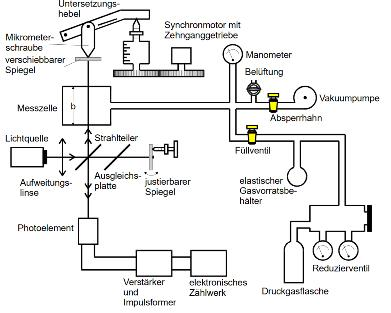
\includegraphics[scale=0.5]{content/images/aufbau.jpg}
\caption{Schematischer Aufbau eines Michelson-Interferometers\cite{V401}}
\label{fig:Aufbau}
\end{figure}

\noindent Der Versuch wird gemäß Abbildung \ref{fig:Aufbau} aufgebaut. Der justierbare Spiegel wird so ausgerichtet, das die am Detektor auftreffenden Strahlen des justierbaren und des verschiebbaren Spiegels
am selben Punkt auftreffen.